\section{Introduction}
\label{sec:intro}

\begin{figure}[t]
	\centering
	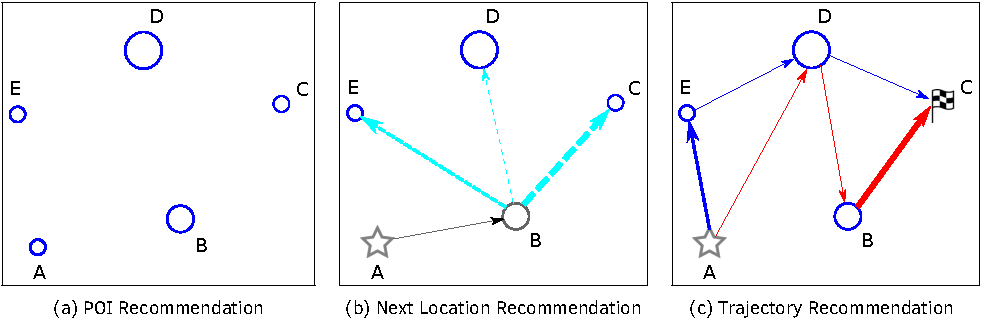
\includegraphics[width=\columnwidth]{fig/fig1-flavours.pdf}
	\caption{Three settings of trajectory recommendation problems.
Node size: POI score; edge width: transition score between pairs of POIs;
grey: observed;
star: starting location; flag: ending location. See Section~\ref{sec:intro} for details.
}
	\label{fig:threesettings}\captionmoveup
\end{figure}


This paper proposes a novel solution to recommend travel routes in cities.
A large amount of location traces are becoming available from ubiquitous location tracking devices.
For example, FourSquare has 50 million monthly users who have made 8 billion check-ins~\cite{4sq},
and Flickr hosts over 2 billion geo-tagged public photos~\cite{flickr}.
This growing trend in rich geolocation data
provide new opportunities for better
travel planning traditionally done with written travel guides.
Good solutions to these problems will in turn lead to better urban experiences for residents and visitors alike, and foster sharing of even more location-based behavioural data.


There are several settings of recommendation problems for locations and routes, as illustrated in Figure~\ref{fig:threesettings}.
We summarise recent work most related to formulating and solving learning problems on assembling routes from POIs,
and refer the reader to a number of recent surveys~\cite{bao2015recommendations,zheng2015trajectory,zheng2014urban} for general overviews of the area.
The first setting can be called POI recommendation (Figure~\ref{fig:threesettings}(a)). Each location (A to E) is scored with geographic and behavioural information such as category, reviews, popularity, spatial information such as distance, and temporal information such as travel time uncertainty, time of the day or day of the week.
A popular approach is to recommend POIs with a collaborative filtering model
on user-location affinity~\cite{shi2011personalized}, with additional ways to incorporate spatial~\cite{lian2014geomf,liu2014exploiting}, temporal~\cite{yuan2013timeaware,hsieh2014mining,gao2013temporal}, or spatial-temporal~\cite{yuan2014graph} information.

Figure~\ref{fig:threesettings}(b) illustrates the second setting: next location recommendation.
Here the input is a partial trajectory (e.g. started at point A and currently at point B), the task of the algorithm is to score the next candidate location (e.g, C, D and E) based on the perceived POI score and transition compatibility with input $A\rightarrow B$.
It is a variant of POI recommendation except both the user and locations travelled to date are given. The solutions to this problem include incorporating Markov chains into collaborative filtering~\cite{fpmc10,ijcai13,zhang2015location},
quantifying tourist traffic flow between points-of-interest~\cite{zheng2012patterns},
formulating a binary decision or ranking problem~\cite{baraglia2013learnext}, and predict the next location with sequence models such as recurrent neural networks~\cite{aaai16}.


This paper considers the final setting: trajectory recommendation (Figure~\ref{fig:threesettings}(c)). Here the input are some factors about the desired route, e.g. starting point A and end point C, along with auxiliary information such as the desired length of trip. The algorithm needs to take into account location desirability (as indicated by node size) and transition compatibility (as indicated by edge width), and compare route hypotheses such as A-D-B-C and A-E-D-C. Existing work in this area either uses heuristic combination of locations and routes~\cite{lu2010photo2trip,ijcai15,lu2012personalized}, or formulates an optimisation problem that is not informed or evaluated by behaviour history~\cite{gioniswsdm14,chen2015tripplanner}.
We note, however, that two desired qualities are still
missing from the current solutions to trajectory recommendation.
The first is a principled method to jointly learn POI ranking (a prediction problem)
and optimise for route creation (a planning problem).
The second is a unified way to incorporate various features
such as location, time, distance, user profile and social interactions,
as they tend to get specialised and separate treatments.
This work aims to address both challenges. 
We propose a novel way to learn point preferences and routes jointly.
In Section~\ref{sec:feature}, we describe the features that are used to ranking points,
and POI to POI transitions that are factorised along 
different types of location properties.
Section~\ref{sec:recommendation} details a number of our proposed approaches to recommend trajectories.
We evaluate the proposed algorithms on trajectories from five different cities in Section~\ref{sec:experiment}.
The main contributions of this work are:
\begin{itemize}
\setlength{\itemsep}{-2pt}
\item We propose a novel algorithm to jointly optimise point preferences and routes. We find that learning-based approaches generally outperform heuristic route recommendation~\cite{ijcai15}.
Incorporating transitions to POI ranking results in a better sequence of POIs, and avoiding sub-tours further improves performance of classical Markov chain methods.
\item Our approach is feature-driven and learns from past behaviour without having to design specialised treatment for spatial, temporal or social information. It incorporates information about location, POI categories and behaviour history, and can use additional time, user, or social information if available.
\item We show good performance compared to recent results~\cite{ijcai15}, and also quantify the contributions from different components, such as ranking points, scoring transitions, and routing.
\item We propose a new metric to evaluate trajectories, pairs-F$_1$, to capture the order in which POIs are visited. Pairs-F$_1$ lies between 0 and 1, and achieves 1 if and only if the recommended trajectory is exactly the same as the ground truth.
\end{itemize}
Supplemental material, benchmark data and results are available online at \surl{https://bitbucket.org/d-chen/tour-cikm16}.
